The starting point to study the relativistic celestial mechanics is to review the formulation of the Keplerian systems using the well known Newtonian gravitational interaction. This is based on the \textit{Poisson equation},
\begin{equation}
\nabla^2 \phi (t, \textbf{x})= 4\pi G \rho (t, \textbf{x}), \label{eq:PoissonEquation}
\end{equation}
where $\phi(t, \textbf{x})$ represents the \textit{gravitational potential} depending on time and space coordinates $\textbf{x} = (x,y,z)$, $G = 6.67 \times 10^{-11} \textrm{ N m}^2\textrm{/kg}^2$ is the Newtonian gravitational constant and $\rho(t, \textbf{x})$ is the matter density. As is shown in Appendix B, a general solution of this equation can be written in terms of the corresponding Green function as
\begin{equation}
\phi (t, \textbf{x}) = -G\int \frac{\rho (t, \textbf{x}')}{\left| \textbf{x} - \textbf{x}' \right|} d^3 x'.
\end{equation}

Considering the case of a point particle with mass $m_1$ as the source in equation (\ref{eq:PoissonEquation}) and due to its spherical symmetry, the general solution is simplified to the potential
\begin{equation}
\phi(r) = - \frac{G m_1}{r}
\end{equation} 
where $r=\left| \textbf{x} \right|$ represents the distance from the particle to the point in space where the potential is evaluated. From this expression, it is also possible to define the \textit{potential energy} stored in a system of two particles with masses $m_1$ and $m_2$ separated by a distance $r$,
\begin{equation}
U(r) = m_2 \phi(r)= -\frac{Gm_1 m_2}{r}.
\end{equation}

Now, we will present the description of a two-body system using Newtonian gravity and the Lagrangian formulation.

\section{The Two-Body Problem}
Consider two point particles with masses $m_{1}$ and $m_{2}$, located at positions 
$\textbf{x}_{1}$ and $\textbf{x}_{2}$ with respect to some coordinate system, as shown in Figure \ref{fig:2BodySystem}.
\begin{figure}[h]
\centering
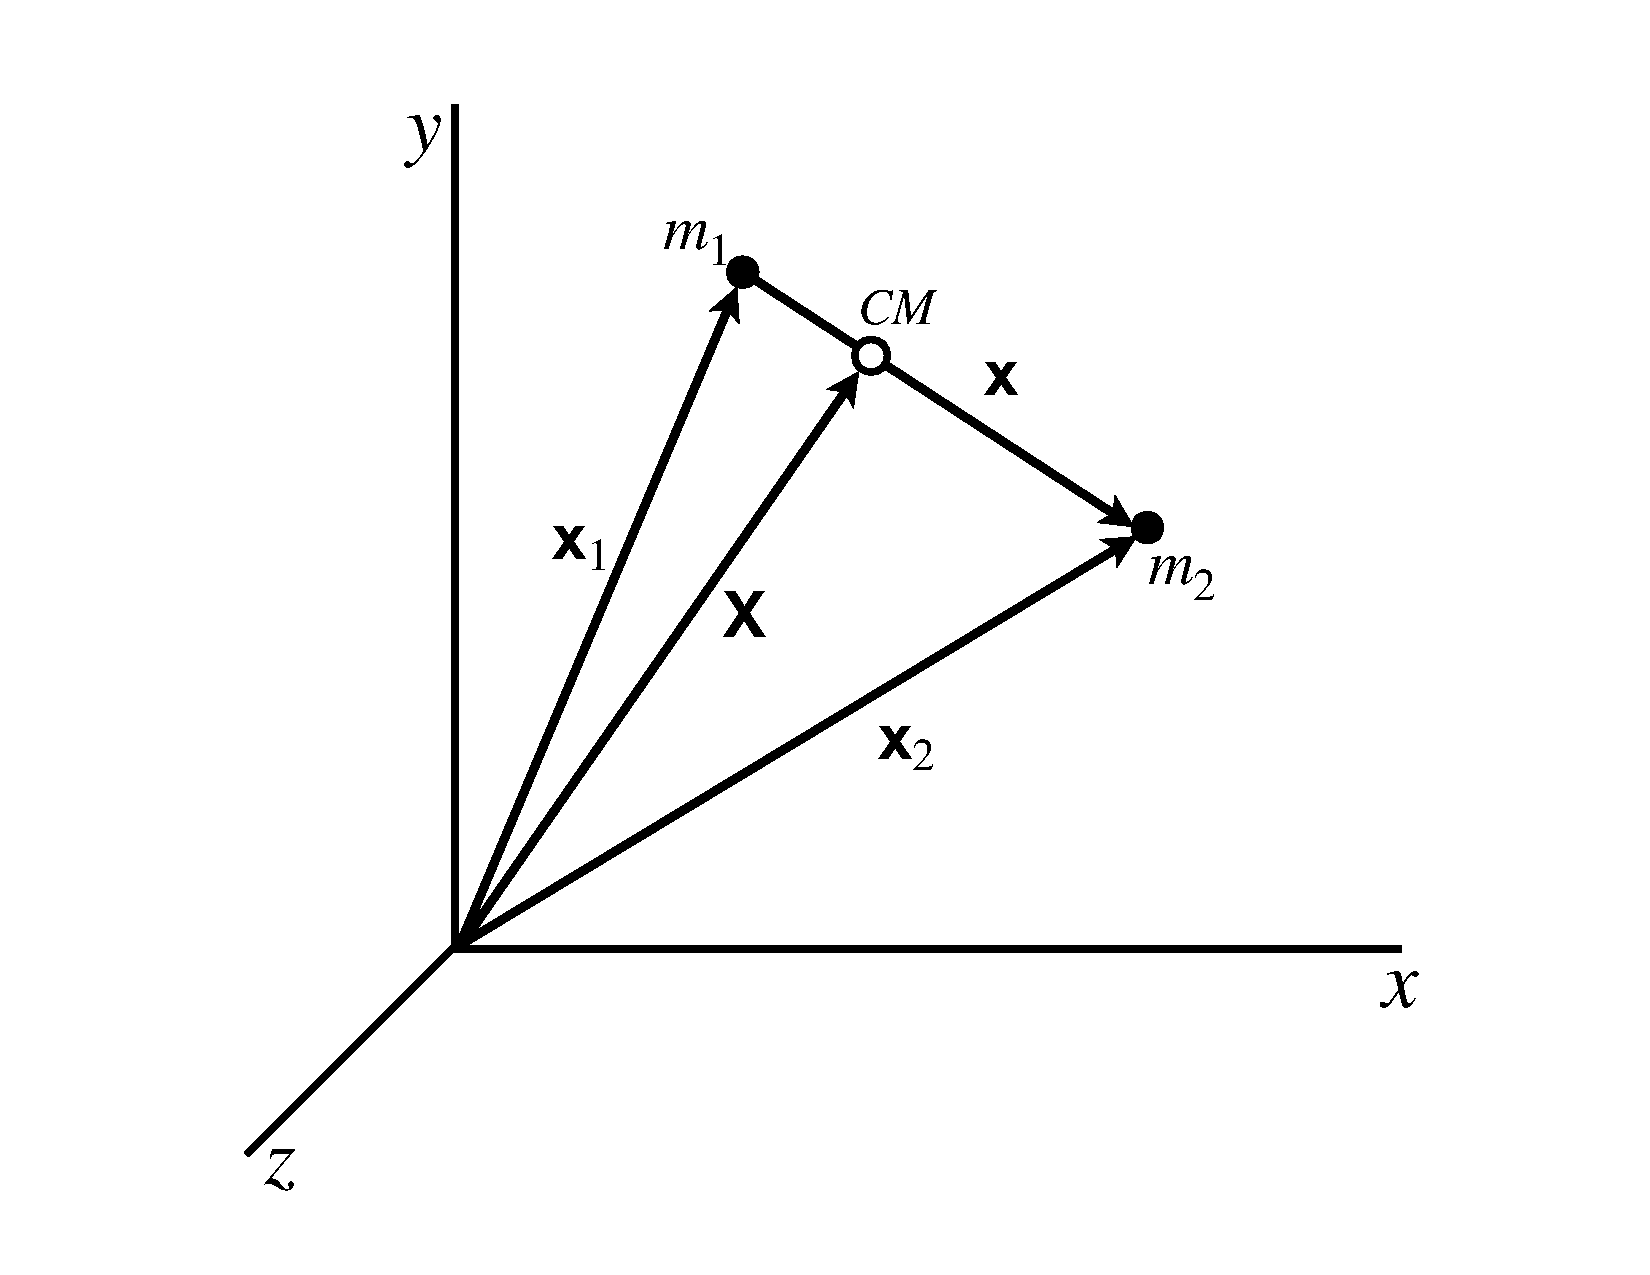
\includegraphics[width=0.6\linewidth]{2BodySystem}
\caption[2-Body System.]
{\label{fig:2BodySystem} Two point particles moving under the mutual gravitational influence. Using the inertial frame shown in the figure, the position vectors of the particles are $\textbf{x}_1$ and $\textbf{x}_2$.}
\end{figure}

We define the relative position vector $\textbf{x}$ through the relation 
\begin{equation}
\textbf{x}=\textbf{x}_{2}-\textbf{x}_{1},
\end{equation}
and thus, the gravitational force between the two point particles can be derived from the potential energy $U\left( r \right) = -\frac{Gm_1 m _2}{r}$. We write the Lagrangian of the two body system as 
\begin{equation}
L=\frac{1}{2}m_{1}\dot{\textbf{x}}_{1}^{2}+\frac{1}{2}m_{2}\dot{\textbf{x}}_2^{2}-U\left( r \right)
\end{equation}
where overdot indicates differentiation with respect to $t$.
Using the center of mass definition,
\begin{equation}
\textbf{X}=\frac{m_{1}\textbf{x}_{1}+m_{2}\textbf{x}_{2}}{M},
\end{equation}
where $M=m_{1}+m_{2}$, the Lagrangian becomes
\begin{equation}
L=\frac{1}{2}M\dot{\textbf{X}}^{2}+\frac{1}{2}\left(\frac{m_{1}m_{2}}{M}\right)\dot{\textbf{x}}^{2}-U\left( r \right).
\end{equation}

This function can be split into two components $L=L_{CM}+L_{rel}$, where $L_{CM}=\frac{1}{2}M\dot{\textbf{X}}^{2}$ is the Lagrangian describing the center of mass and  $L_{rel}$ is the Lagrangian describing the relative  motion of the two particles. It is easily checked that the center of mass will have a uniform rectilinear motion and therefore, we will restrict our attention to the description of the relative motion\footnote{The uniform rectilinear motion of the center of mass provides the definition of an inertial reference system, called \textit{barycentric}, in which the center of mass is located at rest at the origin of the system. We will adopt this system to derive the equations of motion.}. Defining the reduced mass of the system as $\mu=\frac{m_{1}m_{2}}{M}$,  we write the relevant Lagrangian to describe the relative motion as
\begin{equation}
L=\frac{1}{2}\mu\dot{\textbf{x}}^{2} - \mu \phi(r), \label{eq:2BodyLagrangian}
\end{equation}
which can be interpreted as the Lagrangian describing a particle with mass
 $\mu$ moving under the interaction described by the gravitational potential
 \begin{equation}
 \phi(r) = \frac{U(r )}{\mu} = -\frac{GM}{r}.
 \end{equation}
 
 \vspace{0.5cm}
 \begin{exercise}[Equation of Motion for the Two Body System]
 \textbf{Equation of Motion for the Two Body System}
 
 Show that in the barycentric frame and using cartesian coordinates such that $\textbf{x} = (x^1, x^2, x^3)$ the Euler-Lagrange equations
 \begin{equation}
 \frac{d}{dt} \left( \frac{\partial L}{\partial \dot{x}^j} \right) = \frac{\partial L}{\partial x^j}
 \end{equation}
with $j=1,2,3$ yields the equations of motion for the two-body system as
\begin{equation}
\ddot{\textbf{x}} = - \bnabla \phi (r) = - \frac{GM}{r^3} \textbf{x}. \label{eq:2BodyEoM}
\end{equation}
 \end{exercise}
 
 \subsection{Conserved Quantities in the Two-body Problem}

In order to obtain the conserved quantities in the two-body system description, we will consider the usual spherical coordinates $\textbf{x} = (r, \theta, \varphi )$. Hence, the Lagrangian (\ref{eq:2BodyLagrangian}) becomes
\begin{equation}
 L = \frac{1}{2} \mu \left[ \dot{r}^2 + r^2 \dot{\theta}^2  + r^2 \sin^2 \theta \dot{\varphi}^2 \right] + \frac{GM\mu }{r}.
 \end{equation} 

The canonical conjugated momenta are defined as $p_j = \frac{\partial L}{\partial \dot{x}^j}$. From the above Lagrangian it is clear that the $\varphi$ component of the momentum is conserved,
\begin{equation}
p_\varphi = \frac{\partial L}{\partial \dot{\varphi}} = \mu r^2 \sin^2 \theta \dot{\varphi},
\end{equation}
and it is identified with the azimuthal component of the total angular momentum. 
It is also easy to see that the Hamiltonian 
\begin{equation}
H = \sum_{j=1} ^3 p_j \dot{x}^j - L  = \frac{1}{2} \mu \dot{\textbf{x}}^2 - \frac{GM\mu }{r} \label{eq:2BodyHamiltonian}
\end{equation}
is conserved and that it corresponds to the total energy of the system.


The total angular momentum of the two-body system, assuming that the particles have no spin, is given by $\textbf{L} = m_1 \textbf{x}_1 \times \dot{ \textbf{x} }_1 + m_2 \textbf{x}_2 \times \dot{ \textbf{x} }_2 = \mu \textbf{x} \times \dot{ \textbf{x} }$ and it is also a constant of motion, i.e. $\frac{d\textbf{L}}{dt}=0$, due to the fact that the acceleration lies in the radial direction (\ref{eq:2BodyEoM}). 

Since $\textbf{L}$ is constant and orthogonal to both position and velocity vectors, $\textbf{L}\cdot \textbf{x}  = \textbf{L} \cdot \dot{\textbf{x}} = 0$, the motion of the system lies in a fixed plane that is always perpendicular to the total angular momentum. Introducing a coordinate system with unit vectors $\{ \textbf{i}, \textbf{j}, \textbf{k} \}$  in which the orbit lies in the $XY$ plane, we take $\textbf{L}$ along the $Z$-axis to write
\begin{equation}
\textbf{L} = \mu \boldsymbol{\ell}
\end{equation}
where
\begin{equation}
\boldsymbol{\ell} = \textbf{x} \times \dot{ \textbf{x}} = \ell \textbf{k}, \label{eq:2BodyAngularMomentum}
\end{equation}
$\ell = \left| \boldsymbol{\ell} \right| = \left| \textbf{x} \times \dot{\textbf{x}} \right|$ and $\textbf{k}$ is a unit vector in the $Z$-direction. The motion in this plane can be described by taking $\theta=\frac{\pi}{2}$ and using only the polar coordinates $r$ and $\varphi$. Hence, the position vector has components $\textbf{x} = (r \cos \varphi , r \sin \varphi , 0)$, where we are measuring the angle $\varphi$ with respect to the $X$-axis, as usual. 

However, it is usual to introduce a time dependent basis to describe the motion in which the first vector points from particle $1$ to particle $2$, the second vector lies in the orbital plane and is orthogonal to the first one and the third vector points in the $Z$-direction,
\begin{equation}
\begin{cases}
\textbf{n} = \frac{\textbf{x}}{r} =\cos \varphi \textbf{i} + \sin \varphi \textbf{j}   \\
\boldsymbol{\lambda} = -\sin \varphi \textbf{i} + \cos \varphi \textbf{j} \\
\textbf{k} 
\end{cases} \label{eq:2BodyTimeDependentBasis}
\end{equation}

It is easy to show that these vectors satisfy the relations
\begin{subequations}
\begin{align}
\frac{d \textbf{n}}{d \varphi} =& \boldsymbol{\lambda} \\
\frac{d \boldsymbol{\lambda}}{d \varphi} = & -\textbf{n}.
\end{align}
\end{subequations}

\begin{exercise}[Position,Velocity and Acceleration]
\textbf{Position,Velocity and Acceleration Vectors.}

Show that the position, velocity and acceleration vectors in the time-dependent basis are
\begin{subequations}\label{eq:2BodyPositionVelocityAcceleration}
\begin{align}
\textbf{x} =& r \textbf{n} \\
\dot{ \textbf{x}} =& \dot{r} \textbf{n} + r \dot{\varphi} \boldsymbol{\lambda} \label{eq:2BodyVelocity1} \\
\ddot{ \textbf{x}} =& \left( \ddot{r} - r \dot{\varphi} ^2 \right) \textbf{n} + \frac{1}{r} \frac{d}{dt} \left( r^2 \dot{\varphi} \right) \boldsymbol{\lambda}. \label{eq:2BodyAcceleration1}
\end{align}
\end{subequations}
\end{exercise}

Comparison of the acceleration in equation (\ref{eq:2BodyAcceleration1}) with the equation (\ref{eq:2BodyEoM}) yields to the conclusion that the factor $r^2 \dot{\varphi}$ is a constant of motion due to the radial behavior of the gravitational interaction. This conserved quantity corresponds to the angular momentum magnitude,
\begin{equation}
\ell = r^2 \dot{\varphi}. \label{eq:2BodyAngularMomentum}
\end{equation}

Another conserved quantity is the \textit{Laplace-Runge-Lenz vector} (also called the \textit{eccentricity vector} for reasons that we will show below), defined as 
\begin{equation}
\textbf{e} = \frac{\dot{\textbf{x}} \times \boldsymbol{\ell}}{GM} - \textbf{n}. \label{eq:2BodyLaplaceVector}
\end{equation}

Due to its construction, it is clear that 
\begin{equation}
\boldsymbol{\ell} \cdot \textbf{e} = 0,
\end{equation}
i.e. the eccentricity vector lies in the orbital plane. 

\begin{exercise}[Conservation of the Laplace-Runge-Lenz vector]
\textbf{Conservation of the Laplace-Runge-Lenz vector}

Show explicitly that
\begin{equation}
\frac{d \textbf{e}}{dt} = \textbf{0}.
\end{equation}
\end{exercise}

\subsection{Equations of Motion}
The radial equation of motion is easily obtained from the Hamiltonian (\ref{eq:2BodyHamiltonian}) and (\ref{eq:2BodyVelocity1}) together with (\ref{eq:2BodyAngularMomentum}), giving the first order differential equation
\begin{equation}
\frac{1}{2} \dot{r}^2 + \frac{\ell^2}{2r^2}  - \frac{GM}{r} = \mathcal{E},\label{eq:2BodyEnergy}
\end{equation}
where we've defined the total energy per unit mass $\mathcal{E} = \frac{H}{\mu}$. Introducing an effective potential energy,
\begin{equation}
V_{eff} (r) = \frac{\ell^2}{2r^2}  - \frac{GM}{r}
\end{equation}
the radial equation can be written as 
\begin{equation}
\frac{1}{2} \dot{r}^2 = \mathcal{E} - V_{eff} (r). \label{eq:2BodyEoM1}
\end{equation}

Plenty of information about the possible trajectories can be obtained by studying  the function $V_{eff} (r)$. For example, from the plot in Figure \ref{fig:2BodyEffectivePotential} it is possible to note that there exist circular orbits, determined by the condition
\begin{equation}
\left. \frac{dV_{eff}}{dr} \right|_{r=r_c} = 0,
\end{equation}
which gives the value of the orbit radius as $r_c = \frac{\ell^2}{GM}$. By replacing this value in equation (\ref{eq:2BodyEnergy}), we obtain the energy of the particle at the circular orbit,
\begin{equation}
\mathcal{E}_c = -\frac{GM}{2r_c} = -\frac{G^2 M^2}{2\ell^2}. 
\end{equation}

\begin{figure}[h!]
\centering
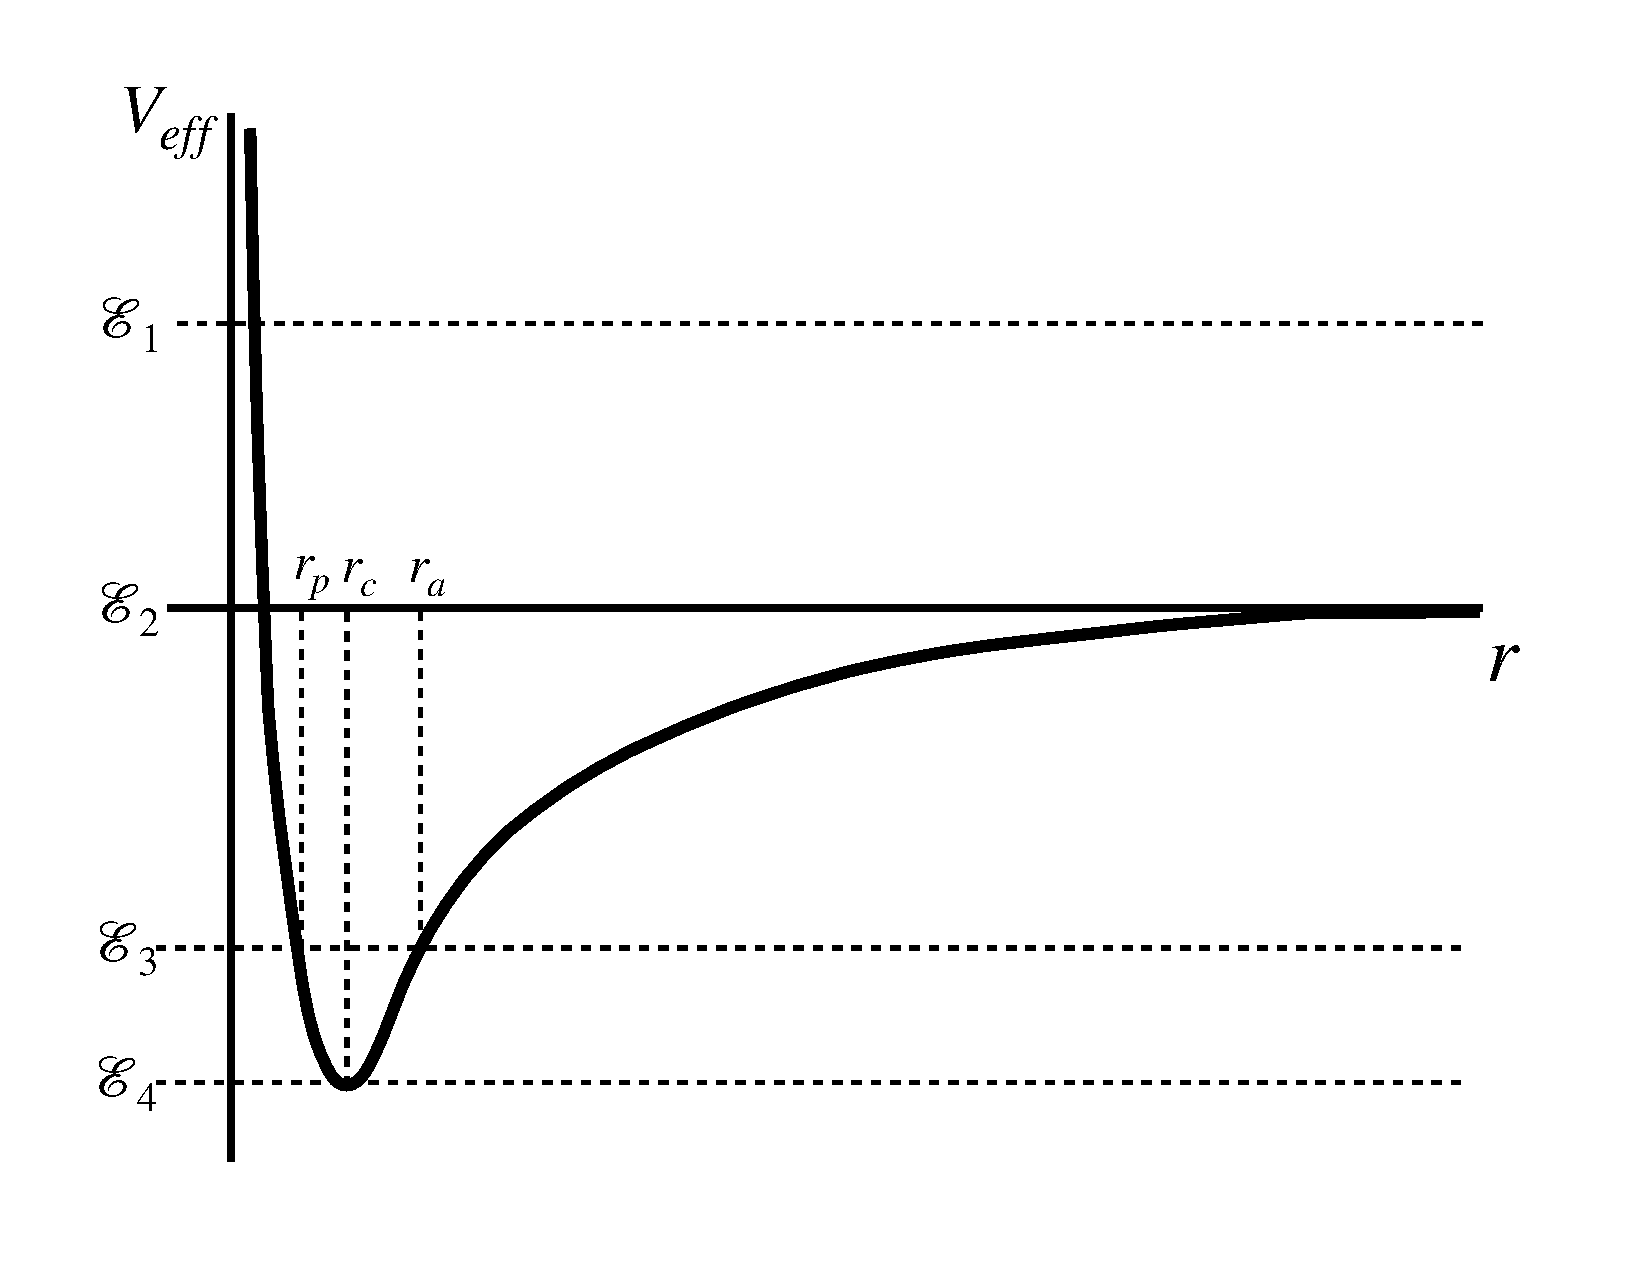
\includegraphics[width=0.6\linewidth]{EffectivePotential}
\caption[Effective Potential for the 2-Body System.]
{\label{fig:2BodyEffectivePotential} Typical behavior of the effective potential for the 2-Body system as function of the separation distance $r$ with $\ell \neq 0$. The horizontal doted lines indicate constant values of the total energy per unit mass $\mathcal{E}$. The motion is allowed only in regions in which $\mathcal{E} \geq V_{eff}$ and thus, intersection of the dotted lines with the effective potential curve correspond to return points in the trajectory. The values $\mathcal{E}_1$ and  $\mathcal{E}_2$ correspond to open trajectories (hyperbolic and parabolic motion). The value $\mathcal{E}_3 < 0$ corresponds to elliptic motion and shows two return points: the pericenter $r_p$ (minimum distance) and the apocenter $r_a$ (maximum distance). The particular value of energy $\mathcal{E}_4 = V_{eff}^{min} $ corresponding to the minimum of the effective potential energy, describes a circular orbit with radius $r_c$. }
\end{figure}

The analytic form of the trajectories can be found by using $\varphi$ as the independent variable instead of the time, i.e. considering $r=r(\varphi)$. It is also usual to introduce a new variable, $u(\varphi)=\frac{1}{r(\varphi)}$. 

\begin{exercise}[Differential Equation of the Trajectory]
\textbf{Differential Equation of the Trajectory}

Show that the second order differential equation of the trajectory obtained from equation (\ref{eq:2BodyEoM1}) and the new variable $u(\varphi)$ is
\begin{equation}
u'' + u = \frac{GM}{\ell^2},\label{eq:2BodyTrayectoryEquation}
\end{equation}
where prime denotes differentiation with respect to $\varphi$.
\end{exercise}

The solution of the differential equation (\ref{eq:2BodyTrayectoryEquation}) are the conic sections
\begin{equation}
r(\varphi) = \frac{p}{ 1 + e \cos (\varphi - \omega ) } \label{eq:2BodyConicEquation}
\end{equation}
where 
\begin{equation}
p = \frac{\ell ^2}{GM} 
\end{equation}
is known as the \textit{semi-latus rectum} of the orbit\footnote{The name \textit{semi-latus rectum} comes from the latin words \textit{semi} (half), \textit{latus} (side) and \textit{rectum} (straight). Geometrically, the \textit{latus rectum} is defined as the length of a chord passing through one focus and perpendicular to the major axis. Therefore, the \textit{semi-latus rectum} is one half of this length.} and $e$ and $\omega$ are constants of integration.The constant $e$ defines to the eccentricity of the trajectory and, since we are interested only in elliptic orbits, we will assume that $0\leq e < 1$. On the other hand, the constant $\omega$ defines the angle $\varphi$ at which $r$ achieves a minimum, and therefore it is called the \textit{longitude of the pericenter}. In fact, when $\varphi = \omega$ we obtain the pericenter radius
\begin{equation}
r_{p} = \frac{p}{1+e}
\end{equation}
while $\varphi=\omega + \pi$ gives the maximum value of the radius or \textit{apocenter},
\begin{equation}
 r_{a} = \frac{p}{1-e}.
 \end{equation} 

From these two values we obtain the \textit{semi-major axis} as
\begin{equation}
a = \frac{1}{2} \left( r_{p} + r_{a} \right) = \frac{p}{1-e^2}.
\end{equation}

Using equations (\ref{eq:2BodyConicEquation}) and (\ref{eq:2BodyAngularMomentum}) we can write the radial velocity as
\begin{align}
\dot{r} &= \sqrt{\frac{GM}{p}} e \sin (\varphi - \omega) \label{eq:2BodyRadialVelocity} 
\end{align}
and replacing this expression in equation (\ref{eq:2BodyEnergy}) gives the energy per unit mass for the elliptic motion as
\begin{equation}
\mathcal{E} = -\frac{GM (1-e^2)}{2p} = -\frac{GM}{2a}.
\end{equation}
Similarly, the angular momentum vector per unit mass in equation (\ref{eq:2BodyAngularMomentum}) can be written as
\begin{equation}
 \boldsymbol{\ell} = \sqrt{GMp} \textbf{k}.
 \end{equation} 
 

\begin{exercise}[Magnitude of the Laplace-Runge-Lenz vector]
\textbf{Magnitude of the Laplace-Runge-Lenz vector}

Show that the Laplace-Runge-Lenz vector for elliptic trajectories can be written as
\begin{equation}
\textbf{e} = e \left[ \cos (\varphi - \omega) \textbf{n} - \sin (\varphi - \omega) \boldsymbol{\lambda} \right] \label{eq:2BodyLaplaceVector2}
\end{equation}
and therefore, this vector always points in the direction of the pericenter of the orbit and its magnitude is equal to the eccentricity of the orbit, $\left| \textbf{e} \right| = e$.
\end{exercise}


\subsection{Time Dependence}\label{sec:TimeDependenceCM}
A formal integration of the energy equation (\ref{eq:2BodyEoM1}) solves the radial problem as a function of time,
\begin{equation}
\int_{r_p}^r \frac{dr}{\sqrt{2[\mathcal{E} - V_{eff} (r)]}} = t - t_p,
\end{equation}
where $t_p$ corresponds to the \textit{time of pericenter passage}. Similarly, using equation (\ref{eq:2BodyAngularMomentum}), it is possible to write the angular velocity as
 \begin{align}
\dot{\varphi} &= \sqrt{\frac{GM}{p^3}} \left[ 1+ e \cos (\varphi - \omega) \right]^2 \label{eq:2BodyAngularVelocity}
\end{align}
and a formal integration of this expression gives
\begin{equation}
\sqrt{\frac{p^3}{GM}} \int_\omega ^\varphi \frac{d\varphi}{\left[ 1+ e\cos (\varphi - \omega) \right]^2} =  t-t_p .
\end{equation}
Note that the lower limit in the integral corresponds again to the passage through the pericenter, located at $\varphi = \omega$. Although these expressions formally solve the motion problem with time dependence, it is usual to use other approach, based on the so-called \textit{Kepler's equation}, to obtain the position of the particle as function of time. 

\subsubsection{Kepler's Equation}

We begin this approach by defining two new variables, the \textit{true anomaly} $f = \varphi - \omega$ and the \textit{eccentric anomaly} $E$. Figure \ref{fig:ReferenceCircleandOrbit} illustrates these angular variables and from the geometry of the plot, it is possible to show that these variables are related through the relations
 \begin{subequations}\label{eq:2BodyEandfRelations1}
 \begin{align}
 \cos E &= \frac{\cos f + e}{1+ e \cos f}\\
 \sin E &= \frac{\sqrt{1-e^2} \sin f}{1+e \cos f}.
 \end{align}
 \end{subequations}
 Equivalently, these expressions can be written as
 \begin{equation}
 \tan \frac{f}{2} = \sqrt{\frac{1+e}{1-e}} \tan \frac{E}{2} \label{eq:2BodyfandErelation}
 \end{equation}
 which clearly states that at the pericenter, $f=0$, the eccentric anomaly is $E=0$. Also note that $e=0$ implies that $f=E$ for circular motion.
 
\begin{figure}[h]
\centering
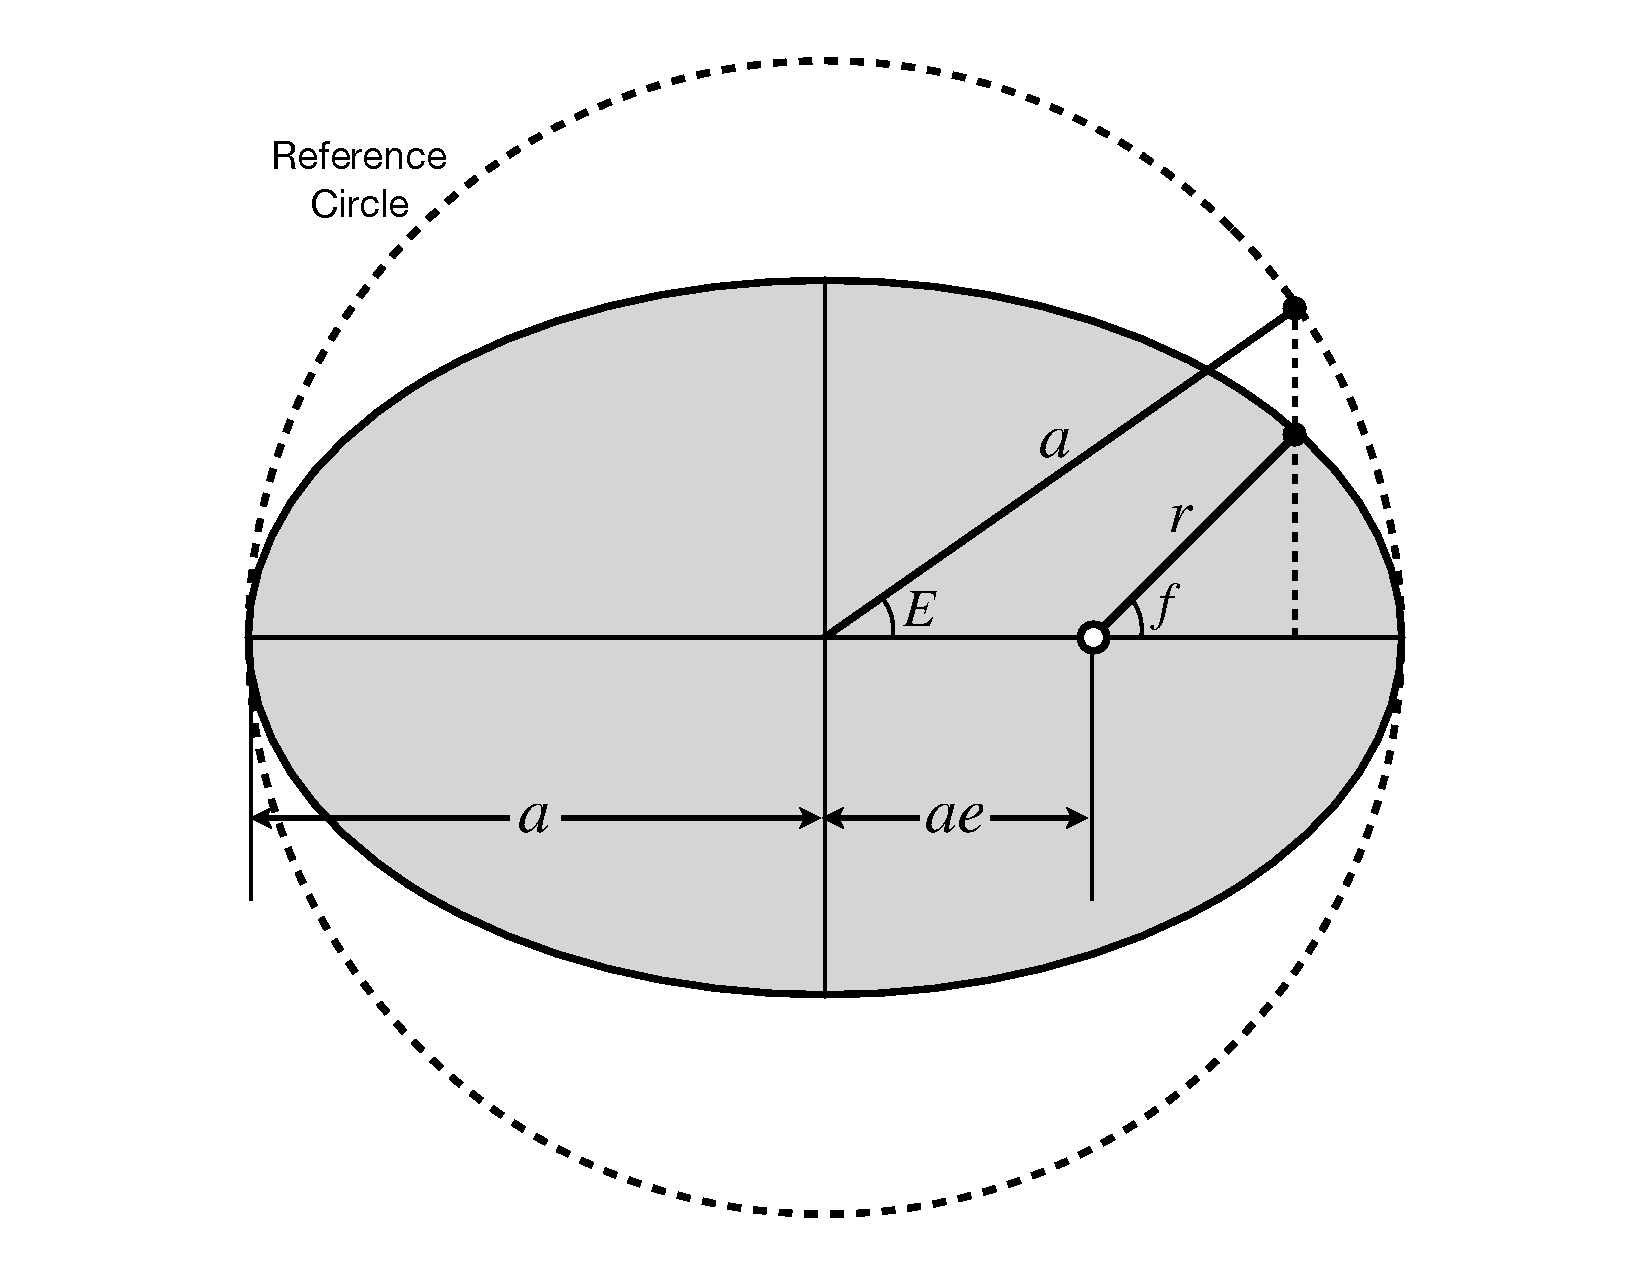
\includegraphics[width=0.7\linewidth]{ReferenceCircleandOrbit}
\caption[Elliptic Orbit in the 2-Body System and the Reference Circle.]
{\label{fig:ReferenceCircleandOrbit} Elliptic orbit in the 2-body problem. The plot indicates some of the geometrical quantities such as the semi-major axis $a$, the relative distance vector $\textbf{r}$ and the true anomaly $f$. It is also shown the \textit{reference circle}, which coincides with the elliptic orbit both at the pericenter and at the apocenter, and the \textit{Eccentric Anomaly}, $E$.}
\end{figure} 

 \begin{exercise}[Eccentric and True Anomalies]
 \textbf{Eccentric and True Anomalies}
 
 Show that equations (\ref{eq:2BodyEandfRelations1}) can be inverted to obtain
 \begin{subequations}\label{eq:2BodyEandfRelations2}
 \begin{align}
 \cos f &= \frac{\cos E - e}{1 - e \cos E}\\
 \sin f &= \frac{\sqrt{1-e^2} \sin E}{1 - e \cos E},
 \end{align}
 \end{subequations}
 and that
 \begin{subequations}\label{eq:2BodyEandfDerivatives}
 \begin{align}
\frac{df}{dE} &= \frac{\sqrt{1-e^2}}{1 - e\cos E}\\
\frac{dE}{df} &= \frac{\sqrt{1-e^2}}{1+e\cos f}.
 \end{align}
 \end{subequations}
 \end{exercise}
 
In terms of the eccentric anomaly, we can write an alternatives set of equations describing the orbit.In particular, equations (\ref{eq:2BodyConicEquation}), \ref{eq:2BodyTrayectoryEquation}) and (\ref{eq:2BodyAngularMomentum}) become
 \begin{subequations}\label{eq:2BodyEquationswithE}
 \begin{align}
 r &= a(1-e\cos E)\\ \label{eq:2BodyPositionwithE}
 \dot{r} &= \sqrt{\frac{GM}{a}} \frac{e \sin E}{1-e\cos E}\\
  \dot{E} &= \sqrt{\frac{GM}{a^3}} \frac{1}{1-e\cos E}. \label{eq:2BodyEderivative}
 \end{align}
 \end{subequations}
 
 Equation (\ref{eq:2BodyEderivative}) is integrated to obtain the transcendental \textit{Kepler's Equation},
 \begin{equation}
l = \sqrt{\frac{GM}{a^3}} \left( t-t_p \right) =  \left( E - e \sin E \right), \label{eq:2BodyKeplerEquation}
 \end{equation}
where we defined  the \textit{mean anomaly}, $l$. Using this equation we can obtain the position at each time as follows: 
\begin{enumerate}
\item Given a time $t$, we invert Kepler's equation to obtain the eccentric anomaly $E(t)$.

\item Then, we use equation (\ref{eq:2BodyfandErelation}) to obtain the true anomaly $f$ which immediately gives the angular position $\varphi(t)$.

\item The radial position $r(t)$ is obtained via equation (\ref{eq:2BodyConicEquation}). 

\item Additionally, we can get the components of the velocity $\dot{r}(t)$ and $\dot{\varphi} (t)$ using equations (\ref{eq:2BodyRadialVelocity}) and (\eqref{eq:2BodyAngularVelocity}).
\end{enumerate}

Kepler's equation also permit us to calculate the period of the orbit because when $E$ goes from $0$ to $2\pi$, time incresases from $t_p$ to the period $T$. This gives
\begin{equation}
T = 2\pi \sqrt{\frac{a^3}{GM}},
\end{equation}
which is exactly Kepler's third law. Using this expression together with Kepler's equation (\ref{eq:2BodyKeplerEquation}) let us write the mean anomaly as
\begin{equation}
l = n \left( t- t_p \right)
\end{equation}
where 
\begin{equation}
n = \frac{2\pi }{T} = \sqrt{\frac{GM}{a^3}}
\end{equation}
is called the \textit{mean motion}. It is also usual to use a reference time  or \textit{epoch}, $t_0 \neq t_p$ such that the mean anomaly is written as the linear function of time
\begin{equation}
l = l_0 + n (t - t_0)
\end{equation}
where $l_0$ is the mean anomaly at the epoch. Note that these expressions imply that for circular motion, $e=0$, all the anomalies coincide, $f=E=l$\footnote{In fact, the name \textit{anomaly} comes from the early belief that circular motion is perfect. Therefore, deviations from perfection, such as elliptic motion, were considered \textit{anomalies}}.

\section{Orbital Elements} \label{sec:OrbitalElements}

\begin{figure}[h]
\centering
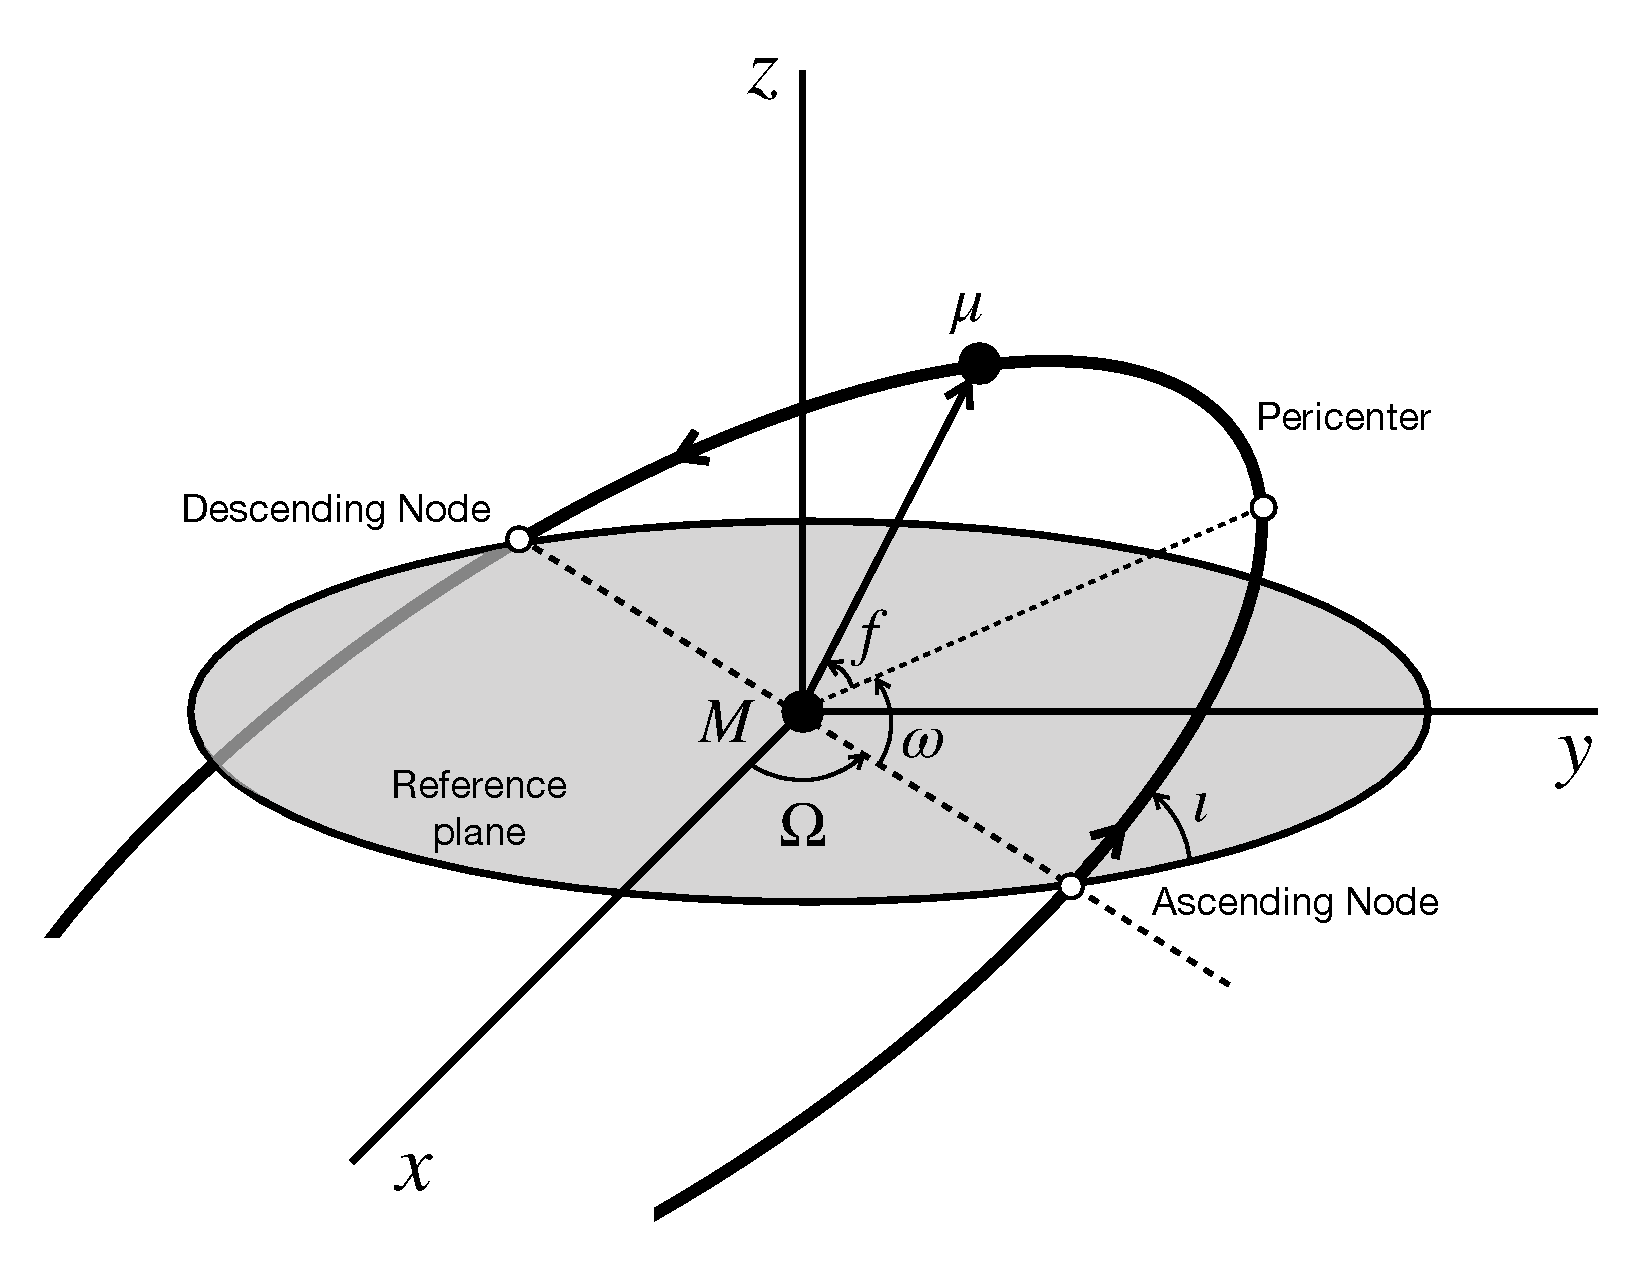
\includegraphics[width=0.7\linewidth]{OrbitalElements}
\caption[Elliptic Orbit in space and Orbital Elements]
{\label{fig:OrbitalElements} Elliptic Orbit in the 2-body problem shown in 3-dimensional space. The orbital elements $\iota$, $\Omega$ and $\omega$ are shown.}
\end{figure}

Until now, we've  been working in the orbit plane and we've defined two basis. The first one corresponds to a barycentric inertial frame with basis vectors $\{\textbf{i}, \textbf{j}, \textbf{k}\}$ while the second uses a time-dependent basis given by the vectors $\{ \textbf{n}, \boldsymbol{\lambda} ,\textbf{k} \}$. Now we will consider a more general coordinate system $(x,y,z)$ in which the orbit is no longer in the $xy$ plane (which will be called now the \textit{fundamental plane}) and we will denote the basis for this new system as $\{\textbf{e}_x, \textbf{e}_y, \textbf{e}_z \}$. 
It is clear that, we will need additional information to completely define the orbit in three-dimensional space. As shown in Figure \ref{fig:OrbitalElements}, we will introduce the \textit{inclination angle}, $\iota$, as the angle between the orbital plane and the fundamental plane\footnote{The inclination can also be defined as the angle between the $z$ axis and the $\textbf{k}$ vector defined before.}.  The line of intersection between the orbital plane and the fundamental plane is called the \textit{line of nodes} and the point along this line in which the trajectory cuts the fundamental plane from below is called the \textit{ascending node}. Also in Figure \ref{fig:OrbitalElements}, it can be seen the angle between the $x$ axis and the line of nodes, which is called the \textit{longitude of the ascending node}, $\Omega$. 

Thus, there are six \textit{orbital elements} or parameters that define completely the orbit,
\begin{itemize}
\item Principal Elements:
\begin{enumerate}
\item $p$ : \textit{Semi-latus rectum}  or $a$ : \textit{Semi-major axis}
\item $e$ : \textit{Eccentricity}
\end{enumerate}
\item Positional Elements:
\begin{enumerate}
\setcounter{enumi}{2}
\item $\omega$ : \textit{Argument of the pericenter}
\item $\iota$ : \textit{Inclination}
\item $\Omega$ : \textit{Longitude of the ascending node}
\end{enumerate}
\item Time element:
\begin{enumerate}
\setcounter{enumi}{5}
\item $T$ : \textit{Orbital period} or $l_0$ : \textit{Mean anomaly at the epoch}.
\end{enumerate}
\end{itemize}

The transformation of a vector $\textbf{A}$, with components $\textbf{A}= A^1 \textbf{i} + A^2 \textbf{j} + A^3\textbf{k}$ in the barycentric frame, to the fundamental coordinate system, in which its components will be denoted $\textbf{A}= A^x \textbf{e}_x + A^y \textbf{e}_y + A^z\textbf{e}_z$, can be represented as
\begin{equation}
 \left( \begin{array}{c}
 A^x \\
 A^y \\
 A^z
 \end{array}  \right) = R_3 (\Omega)  R_1 (\iota) R_3 (\omega) 
 \left( \begin{array}{c}
 A^1 \\
 A^2 \\
 A^3
 \end{array} \right), \label{eq:2BodyCoordinatesTransformation}
 \end{equation} 
 and involves three rotations matrices,
\begin{subequations}
\begin{align}
R_3 (\omega) &= \left( \begin{array}{c c c}
\cos \omega & -\sin \omega & 0 \\
\sin \omega & \cos \omega & 0 \\
0 & 0 & 1
\end{array} \right) \\
R_1 (\iota) &= \left( \begin{array}{c c c}
1 & 0 & 0 \\
0 & \cos \iota & - \sin \iota \\
0 & \sin \iota & \cos \iota
\end{array} \right) \\
R_3 (\Omega) &= \left( \begin{array}{c c c}
\cos \Omega & -\sin \Omega & 0 \\
\sin \Omega & \cos \Omega & 0 \\
0 & 0 & 1
\end{array} \right).
\end{align}
\end{subequations}

For example, the vectors of the time dependent basis (\ref{eq:2BodyTimeDependentBasis}) written now in terms of the true anomaly,
\begin{equation}
\begin{cases}
\textbf{n} =\cos f \textbf{i} + \sin f \textbf{j}   \\
\boldsymbol{\lambda} = -\sin f \textbf{i} + \cos f \textbf{j} \\
\textbf{k} 
\end{cases} \label{eq:2BodyTimeDependentBasisinf}
\end{equation}
can be transformed using (\ref{eq:2BodyCoordinatesTransformation}) to obtain their components in the fundamental coordinate system,
\begin{subequations}\label{eq:timeDepBasis}
 \begin{align}
 \textbf{n} = & \left[ \cos \Omega \cos (f + \omega) - \cos \iota \sin \Omega \sin (f + \omega) \right] \textbf{e}_x \notag \\
 & + \left[ \sin \Omega \cos (f + \omega) + \cos \iota \cos \Omega \sin (f + \omega) \right]\textbf{e}_y \notag \\
 & + \left[ \sin \iota \sin (f + \omega) \right] \textbf{e}_z \\
 \boldsymbol{\lambda} = & \left[ - \cos \Omega \sin (f + \omega) - \cos \iota \sin \Omega \cos (f + \omega) \right] \textbf{e}_x \notag \\
 & + \left[ - \sin \Omega \sin (f + \omega) + \cos \iota \cos \Omega \cos (f + \omega) \right]\textbf{e}_y \notag \\
 & + \left[ \sin \iota \cos (f + \omega) \right] \textbf{e}_z \\
\textbf{ k} = & \sin \iota \sin \Omega \textbf{e}_x - \sin \iota \cos \Omega \textbf{e}_y + \cos \iota \textbf{e}_z .
 \end{align}
 \end{subequations} 
 
The first of these relations gives immediately the components of the separation vector, because $\textbf{x} = r \textbf{n}$ with $r = \frac{p}{1+e\cos f}$. Denoting the components of this vector in the fundamental system as $\textbf{x} = (x,y,z)$, we have 
 \begin{equation}
 \begin{cases}
 x &= r \left[ \cos \Omega \cos (f + \omega) - \cos \iota \sin \Omega \sin (f + \omega) \right] \\
 y &= r \left[ \sin \Omega \cos (f + \omega) + \cos \iota \cos \Omega \sin (f + \omega) \right] \\
 z &= r \sin \iota \sin (f + \omega),
 \end{cases}
 \end{equation}
and differentiating with respect to time we obtain the components of the relative  velocity, $\dot{\textbf{x}}$, in the fundamental frame,
\begin{equation}
 \begin{cases}
 \dot{x} &= -\sqrt{\frac{GM}{p}} \left[ \cos \Omega \left( \sin (f + \omega) + e \sin \omega \right) + \cos \iota \sin \Omega \left ( \cos (f + \omega) + e \cos \omega \right) \right] \\
 \dot{y} &= -\sqrt{\frac{GM}{p}}  \left[ \sin \Omega \left( \sin (f + \omega) + e \sin \omega \right) - \cos \iota \cos \Omega \left ( \cos (f + \omega) + e \cos \omega \right) \right]\\
 \dot{z} &= \sqrt{\frac{GM}{p}}  \sin \iota \left[ \cos (f + \omega) + e \cos \omega \right].
 \end{cases}
 \end{equation}

Another interesting transformation is to obtain the components of the eccentricity vector in the fundamental coordinate system. Replacing the basis vectors (\ref{eq:timeDepBasis}) in equation (\ref{eq:2BodyLaplaceVector2}) gives
 \begin{align}
\textbf{e} = e \left[ \right.& \left( \cos \Omega \cos \omega - \cos \iota \sin \Omega \sin \omega \right) \textbf{e}_x \notag \\
& + \left( \sin \Omega \cos \omega + \cos \iota \cos \Omega \sin \omega \right)\textbf{e}_y \notag \\
& + \left( \sin \iota \sin \omega \right) \textbf{e}_z \left. \right].
 \end{align} 
 
 All these equations let us write the set of orbital elements through the relations
 \begin{subequations}\label{eq:2BodyOrbitalElements}
 \begin{align}
 p &= \frac{\ell^2}{GM} \\
 a &= \frac{p}{1-e^2} \\
 e &= \left| \textbf{e} \right| \\
 \cos \iota &= \textbf{k} \cdot \textbf{e}_z \\
 \sin \iota \sin \Omega &= \textbf{k} \cdot \textbf{e}_x \\
 \sin \iota \sin \omega &= \frac{\textbf{e} \cdot \textbf{e}_z}{e} .
 \end{align}
 \end{subequations}
 
 \iffalse
 \section{Problems}
 
 \textbf{Sun-Jupiter System}
 
 In this problem, we will consider only the two-body system Sun-Jupiter, ignoring other interactions and corrections.
 
 \begin{enumerate}
 \item The semi-major axis and the eccentricity of Jupiter are $a=5.2044 \textrm{ A.U.}$ and $e=0.0489$ and it has a mass of $m_J = 0.0009543 M_{\odot }$ \cite{JupiterData}. Considering only the two-body system Sun-Jupiter, obtain the following characteristics for Jupiter:
 \begin{enumerate}
 \item Distance to the Sun at the perihelion.
 \item Distance to the Sun at the aphelion.
 \item Orbital period.
 \item Semi-latus rectum.
 \item Speed at the perihelion.
 \item Mean motion.
 \end{enumerate}
 
 \item Consider the position of Jupiter when its true anomaly has the value $f=\frac{2\pi}{3}$. 
 \begin{enumerate}
 \item Calculate the distance Sun-Jupiter at this point.
 \item At the moment in which Jupiter is at this point, how much time has passed since its nearest pass through its perihelion ?
 \item Obtain the values of the eccentric anomaly and the mean anomaly at this point.
 \end{enumerate}
 \end{enumerate}
 
 \textbf{Earth-Moon System}
 
 In this problem we will consider only the two-body system Earth-Moon, ignoring other interactions and corrections.
 \begin{enumerate}
 \item The mass of the Moon is $m_{Moon} = 0.012300 M_{Earth}$. Find the location of the center of mass of the system as measured from the center of the Earth.
 \end{enumerate}
 \fi